
\chapter{Embedded ML Infrastructure for Plasma Characterization}
\label{section:4_embedded_ML}

It has been shown in the introductory chapter the diversification of signals within their heterogeneous nature, however a particular discussion should be also addressed to the possible domain of the data itself beyond the particular origin.
In order to provide high quality descriptions of the plasma properties during a the pulse in a fusion experiment session a wide amount of sensors are usually required, both in time and in spatial domains.
Although it is not true that controllability (and observability) of the system strictly depends on that amount of inputs; the overall description of a complex system, indeed, is usually led by few driving signals~\cite{Liu2011}. 
This definition agrees with the intuitive notion of control that, for a properly structured system, the appropriate manipulation of a few state variables are a sufficient information to drive the whole behavior; like in the bike riding example where the actual only two control variable are the steering of the handlebar and the torque on the pedals. Even if the complete environment of all the variables that must be observed to provide a optimal control on the system states is rather complex, it can be shown that a properly configured latent variables can effectively generate a simpler embedded representation. This in turn leads to a simpler control model taking inputs from the latent states instead of directly depending on the whole detectors.

% CONTROL THEORY
According to the classical \textit{control theory} for dynamical systems, once the precise time derivative description is given in terms of that state space model, a system can be defined \textit{controllable} if there exist a particular set of inputs that are able to drive the state to any desired \textit{set point} within a finite time. 
If the classical discreet time \acl{LTI} state space model is considered in the form:
\begin{align}
    & \dot{\bm{x}} = A\bm{x} + B\bm{u} + \bm{w}\\
    & \bm{y} = C\bm{x} + D\bm{u} + \bm{v}
    \label{eq:ss_model}
\end{align}
% \begin{align}
%     & \bm{x}_t = A\bm{x}_{t-1} + B\bm{u}_t + \bm{w}_t\\
%     & \bm{y}_t = C\bm{x}_t + D\bm{u}_t + \bm{v}_t
%     \label{eq:ss_model}
% \end{align}

Time dependent state space models in \eqref{eq:ss_model}, also known \acl{DLM}, are a widely used approximation for analyzing time series. They provide a very flexible framework allowing concurrent smooth and steep changes that generally well fitting natural process time evolution.
A more rigorous formulation for \textit{controllability} is given in terms of the \textit{Kalman criterion}:
\begin{definition}{Kalman criterion}
The pair $(A,B)$ is \textit{controllable} if, given a duration $t>0$ and two arbitrary points $x_0, x_t \in \mathbb{R}^n$, there exists a piece wise continuous function $\tau \mapsto u(\tau)$ from $[0,t]$ to $\mathbb{R}^m$, such that the integral $x(\tau)$ generated from input $u$ with $x(0) = x_0$, satisfies $x(t)=x_t$.
\end{definition}
Where, as stated, the definition can be formulated in terms of the integral:
\begin{equation}
    e^{A t}x_0 + \int_0^t e^{A(t-\tau)}B u(\tau) d\tau = x_t
\end{equation}
where the only dependencies are on the state and input matrices $A$ and $B$.
Given the definition is well known that for such models the \textit{controllability} and the \textit{observability} depend on the \textit{Kalman condition}:
\begin{equation}
    \mathrm{rank}\,\mathscr{C} = \mathrm{rank}\left( B|AB|...|A^{n-1}B \right) = n
\end{equation}
% It can be shown that once a system is proved to be controllable can be transformed to a system in \textbf{canonical form} where all 

%% Structural Controllability
Recently, the study of the such complex networks with linear dynamics control has gained importance in both science and engineering. Between different aspects in which we can study the controllability we have the notion of structural controllability that has been proposed by Lin in~\cite{1100557} as a framework for studying the controllability properties of directed complex networks where
% LIN
%% RR
% To do this, the basic concept of a "cactus" and the related concept of a "precactus" are introduced. The main result of this paper states that the pair (A,b) is structurally controllable if an only if the graph of (A,b) is "spanned by a cactus." The result is also expressed in a more conventional way, in terms of some properties of the pair (A,b).

% \cite{zheng2017state}
State space models (SSMs), such as hidden Markov models (HMM) and linear dynamical systems
(LDS), have been the workhorse of sequence modeling in the past decades From a graphical model
perspective, efficient message passing algorithms (Stratonovich, 1960; Kalman, 1960) are available
in compact closed form thanks to their simple linear Markov structure. However, simplicity comes
at a cost: real world sequences can have long-range dependencies that cannot be captured by Markov
models; and the linearity of transition and emission restricts the flexibility of the model for complex
sequences.

As a first attempt the simple \textit{Elman} formulation for the recurrent topology will be applied, this with the aim at demonstrating the connection with linear dynamical systems, showing that such networks represent a superset.
With the \textit{Elman} forumlation a \acs{RNN} is control dynamical system that, in continuous time, can be described by a system of differential equations:
\begin{align}
    & \dot{\bm{x}} = \sigma_x \left( A\bm{x} + B\bm{u} \right) \\
    & \bm{y} = C\bm{x}
\end{align}
where for simplicity we omitted noise components for both the state and the output, and the direct input/output link.
% why



A popular alternative is the recurrent neural networks (RNN), for instance the Long Short-Term
Memory (LSTM) (Hochreiter  Schmidhuber, 1997) which has become a standard for sequence
modeling nowadays. Instead of associating the observations with stochastic latent variables, RNN
directly defines the distribution of each observation conditioned on the past, parameterized by a
neural network. The recurrent parameterization not only allows RNN to provide a rich function
class, but also permits scalable stochastic optimization such as the backpropagation through time
(BPTT) algorithm. However, flexibility does not come for free as well: due to the complex form of
the transition function, the hidden states of RNN are often hard to interpret. Moreover, it can require
large amount of parameters for seemingly simple sequence models (Zaheer et al., 2017).



\section{Easing the curse of dimensionality by disentangled factors}


\section{A new “smart” DAQ chain proposal}
% smart sensory
% feature extraction concept

In order to collect magnetic field measurements from EM probes, analog integration system~\cite{pomaro2005transducers} was implemented in RFX-mod, followed by two separate sets of ADC channels, one for precision off-line transient data and the other for real-time control. Re-implementing the same front-end for an increased number of channels is costly, requiring enhanced analog integration and duplication in ADC channels.  A more compact and cost effective solution is being investigated~\cite{gottardo18}, using a configurable FPGA to handle ADC conversion and providing a set of on-line functions directly performed at the FPGA logic level, including the numeric integration in real-time, recording at the same time the dB/dt signals deriving directly from EM coils needed to study the Magneto Hydro Dynamic (MHD) processes taking place into the plasma~\cite{zuin2009current}~\cite{innocente2014tearing}. The possibility of directly acquiring the time derivative of the electromagnetic fields, i.e. the direct signals from EM probes, was not present in the previous system, acquiring integrated signals in order to reduce the number of required ADC channels. This fact introduced a severe limitation in the derivative control required for MHD stabilization because of the bad quality of the computed time derivative.

The proposed approach will further reduce the number of ADC channels by merging high frequency transient recording in local memory (up to 1 MHz) and lower frequency streaming (up to 10 kHz) required for real-time plasma control and having a single ADC channel performing both. In RFX-mod a fixed subset of signals from EM probes was used for the active plasma control, requiring a new set of ADC converters in respect to the transient recorders used for data acquisition. In RFX-mod2 it will be possible to re-use any ADC channel from EM probes for real-time plasma control, being the actual number possibly limited by other factors not related to the ADC devices, such as network bandwidth or control computation load. 
%
The flexibility provided by a configurable on board FPGA allows also the inclusion of more sophisticated triggering mechanisms and a deeper integration with the timing systems. Examples of triggering mechanism are given by the acquisition of fast transients requiring high speed sampling only in a given, dynamic Region of Interest (ROI). This feature has been implemented in the first proof-of-concept device described in a later section. Deeper integration with the timing systems imply the ability of getting the clock and the trigger signals not only from digital inputs, but also from the specifically coded signal carrying both clock and trigger information (timing highway)\cite{dio4}. Such signals were used in the RFX-mod timing systems to distribute a synchronous clock and asynchronous triggers and a timing device was required for every ADC rack to extract the clock and the trigger signals. The timing device is no more required for a rack hosting the new ADC devices because the ADC devices can directly extract timing information from the timing highway.  
%
The adoption of a System on Chip (SoC) based technology exploiting both an ARM based processing unit and a FPGA logic provides the  flexibility of a configurable device for real-time operations and as well as the possibility of deploying software components directly on-board. The Red Pitaya board~\cite{redpitaya} is currently used for the development of the architecture. A different solution is however foreseen for the production system integrating an external ADC section with the Zynq-based SoC board. An ADC front end, already used in other applications of real-time plasma control~\cite{ATCA-MIMO-ISOL} was initially considered, but its noise characteristics, and in particular the noise dependency on frequency, proved to limit the quality of digital integration. For this reason, a different solution for the ADC stage is being considered.

The first implementation of the flexible ADC architecture has been carried out on a Red Pitaya board, using the in-board ADC channels. Even if not intended to represent the final application, development of FPGA logic on Red Pitaya offers the advantage of a ready-to-use ADC channel for development and first tests. Most of the firmware will be retained in the final implementation, using a different ADC front end. 
%
The time critical functions carried out by the FPGA in this context are:
\begin{itemize}
\item The management of a circular data buffer and the DMA transfer in RAM of pre and post trigger samples after the trigger has been received;
\item anti-aliasing filtering and subsequent sub-sampling of the samples to be streamed. The resulting samples are enqueued in a FIFO accessed by the processor;
\item digital integration for deriving magnetic field measurements from EM probe signals. Observe that in this case a single ADC stage will generate two ADC channels;
\item ROI detection in case ADC triggers are derived from the signal itself (e.g. over a given signal level threshold);
\item Clock and trigger extraction in case a highway signal is provided by the timing system, encoding both clock an triggers.
\end{itemize}
%
The less critical functions that will be carried out by the processor unit are:
\begin{itemize}
\item The management of the configuration setting, received via TCP/IP or HTTP. The processor validates the configuration and write the appreciate registers in the FPGA;
\item off-line data readout of acquired samples in transient recording and communication via TCP/IP with the central data acquisition system;
\item network data streaming of sub-sampled data read from the FIFO and sent in UDP packets to the active plasma control system. 
\end{itemize}
%
In addition to pre-configured blocks from the XILINX toolbox for data buffering, DMA engine, I/O FIFO and registers, three blocks implemented in VHDL carry out the underlying logic. The first block provides the management of clock and triggers that may be either directly derived from digital inputs or rebuild by properly decoding the timing highway input signal. The second block provides programmable input signal elaboration such as low pass filtering for subsampling and integration. The third block will handle the triggering logic and the circular buffer holding pre and post trigger samples. In particular, the trigger may be derived from external signals (via the first block) or derived from the input signal (e.g. when the input level is greater than a given threshold).    

Communication of subsamples streamed data for real-time plasma control is achieved using the XILINX AXI Stream FIFO. The Xilinx AXI Stream FIFO is a Xilinx free software IP that implement a read/write FIFO queue with a well defined communication protocol. A proper connected IRQ line is used to trigger events to the processing unit together with the related set of status and enable registers. In this way data samples are readily available to the linux processor and will be sent using low latency UDP communication to computing nodes carrying out distributed for real-time plasma control. Communication of the data acquired at high speed in the ROI is carried out by a DMA engine, using circular DMA buffers in order to minimize the number of data copies. In this case data will be sent to the central Data Acquisition system via TCP/IP as soon as a ROI has been acquired. Fig. 1 shows the main blocks of the ADC device: the external ADC circuitry, communicating with the FPGA via a serial LVDS link; the FPGA logic, communicating with the processor via registers, FIFO and DMA; the processor components, in kernel and user space. 
~
~
\begin{figure}[ht]
\centering
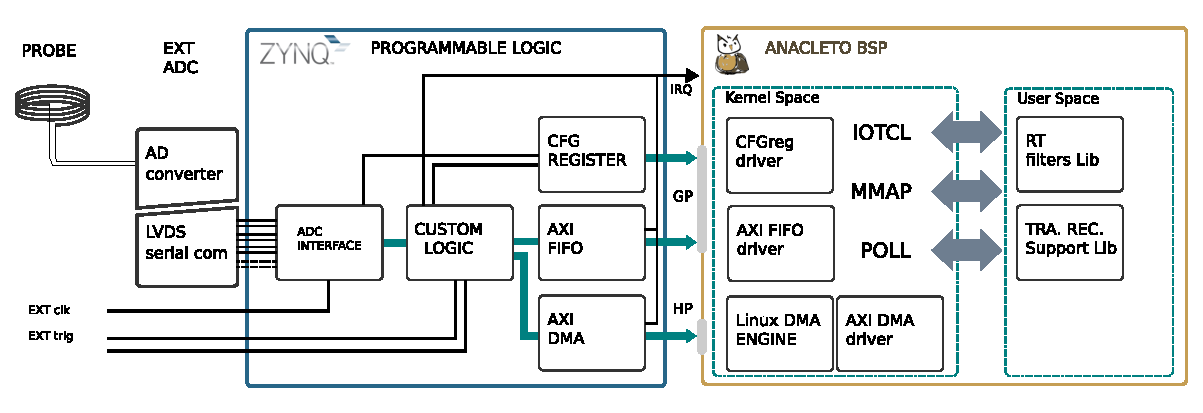
\includegraphics[width=0.9\textwidth]{img/4_EmbeddedML/schema_logico.pdf}
\caption{Logic design of the flexible ADC structure.}
\label{fig:logic}
\end{figure}









\section{Quantized neural networks for embedded implementation}

In numerical computation we refer to the \textit{quantization} as the process of constraining the number of bit that reproduce a numerical value. In effect any digital number is already intrinsically quantized, in the sense that its representation is defined on a limited discreet domain. Nevertheless, even if the number of bits that are used to represent a digital quantity is finite, and so is the possible set of values that it can assume, the actual position of those values in the target domain is not strictly fixed. This means that we can decide where to place any of possible available reproduction number to fit the desired manifold.
If the function that maps the digital representation with a numerical entity is linear the numerical format can be described by only two parameters: the \textbf{range}, which refers to the range of all possible numbers that can be represented, and the \textbf{precision} that tells how many values can be represented within the dynamic range, which in turn determines the resolution (the distance in the target domain between two adjacent numbers).

In the context of deep learning, and in information theory in general, the predominant numerical format used for both training and final deployment is the floating point, either in 32-bits or 64-bits versions. For a \acs{MLP}, for example, floating point operations involves the linear combination of weights and biases with input features for each layer, and the non-linear activation function. The formulation of floating point numerical format is a very clever solution that adapt the range to the represented number.

Floating-point can be thought in concept similar to the scientific notation. Their numbers consist of a signed set of digits of a fixed length in a given base (the radix), this is referred as the \textit{significand}; where its length determines the precision to which numbers can be represented. The radix point position is assumed always to be within the significand, while a signed integer exponent modifies the magnitude of the number.
To finally derive the actual value of the floating-point number the significand is multiplied by the base and raised to the power of the exponent; this is shifting the radix point from its implied position by a number of places equal to the value of the exponent to the right if the exponent is positive or to the left if the exponent is negative.
%
Symbolically, this represented value can be derived as:
\begin{equation*}
    \frac{s}{b^{p-1}} \times b^e
\end{equation*}
where $s$ is the significand, $p$ is the precision (the number of digits in the significand), $b$ is the base, and $e$ is the exponent.
The flexibility introduced by floating point dynamic range is that the numbers that can be represented are not uniformly spaced; the difference between two consecutive representable numbers grows with the chosen scale.

However given this dynamic mapping of the scale the floating point may require a slight amount of computational resources.
When a processing unit is executing an algorithm where a floating-point operation is not directly supported by the hardware, the CPU tries to use a series of simpler floating-point operations, either by basic internal routines or by means of specific libraries. In systems without any floating-point hardware, the CPU emulates it using a series of simpler fixed-point arithmetic operations that run on the integer arithmetic logic unit.
Moreover, being the target a possible FPGA implementation, the full IEEE 754 floating point shown to use a lot of hardware resources in terms of LUTs counts. 

The desire for reduced bandwidth and compute requirements of deep learning models has driven research into using lower-precision numerical formats. It has been largely proved that both linear combination and non linear activation can be effectively represented using a fixed point math, in particular 8-bit integers (INT8) have been successfully applied without incurring in significant loss of accuracy. 
But, not enough, the use of even lower bit-widths, such as 4/2/1-bits, is an active field of research that has also shown great results.

